\begin{frame}{Project Overview}

\textbf{Objectives:}
  \begin{itemize}
    \item Fastest checkmate against optimal player in KRk endgame
    \item Compare different Reinforcement Learning approaches
    \item Assess performance against different opponents (oracle and dummy)
  \end{itemize}

\end{frame}

\section{Chess Programming Background}
\begin{frame}
  \begin{itemize}
    \item 1890 El Ajedrecista: electro-mechanical KRK solver 
    \item 1950 Claude Shannon: first article about chess programming
    \item 1997 \textit{Deep Blue}: first computer program to beat the current world champion
    \item 2008 \textit{Stockfish}: strong heuristic-based chess engine
    \item 2017 \textit{Alphazero}: neural network-based approach that defeated Stockfish
    \item from 2018: more models developed based on \textit{Alphazero}
  \end{itemize}
\end{frame}

\begin{frame}{Chess Rules}
\begin{figure}
  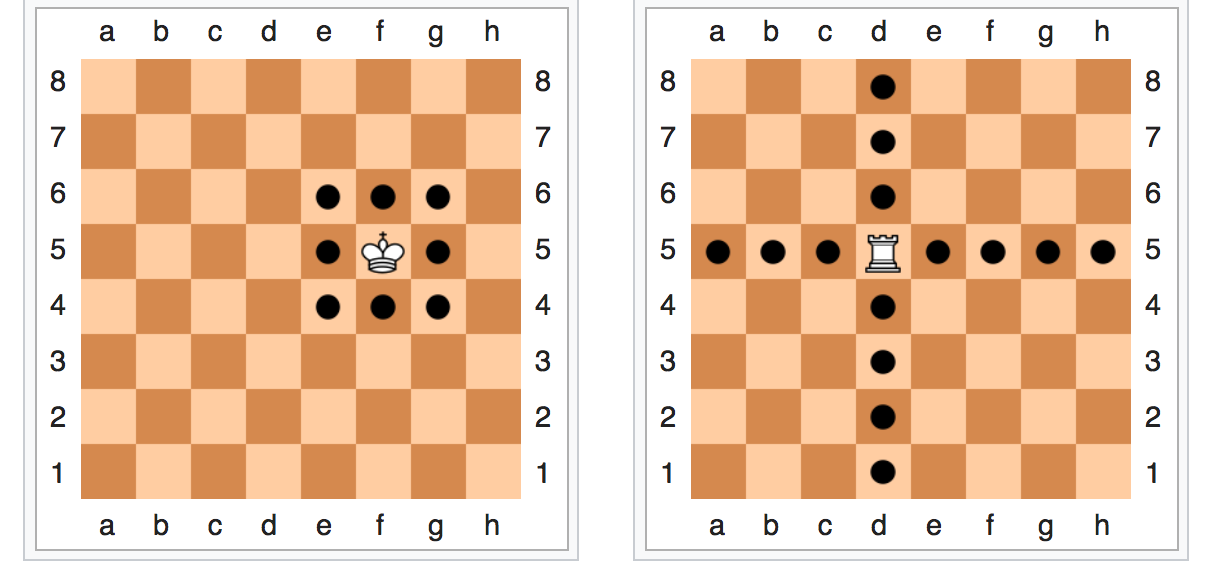
\includegraphics[width=0.8\textwidth]{images/chess-moves.png}
\end{figure}

  \begin{itemize}
    \item \textbf{Win}: checkmate the opponent's king
    \item \textbf{Draw}: stalemate or insufficient material\footnote{\tiny{threefold repetition and the fifty-move rule are not considered in our implementation}}
  \end{itemize}

\end{frame}

\begin{frame}{Elementary Endgames}
\begin{columns}[T]
  \begin{column}{0.6\textwidth}
    \begin{itemize}
      \item subset of endgames with few pieces left
      \item foundation for learning more complex endgames
      \item clear theoretical results: forced checkmate or draw
      \item Sygyzy endgame tablebases
    \end{itemize}
  \end{column}
  \begin{column}{0.4\textwidth}
    \begin{figure}
      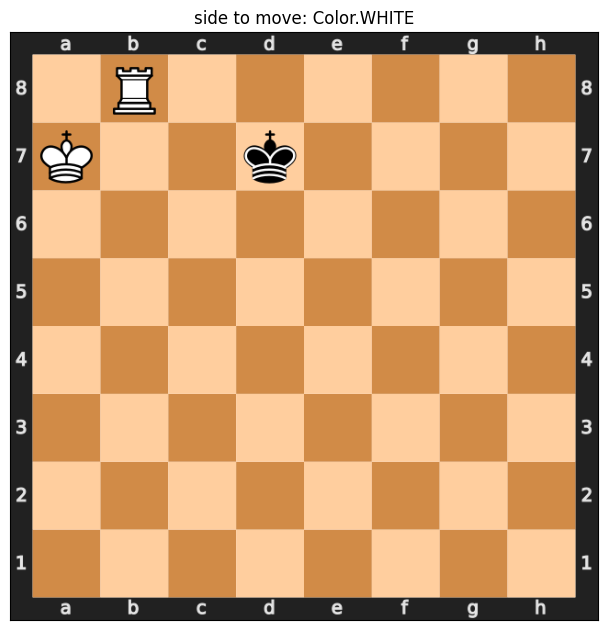
\includegraphics[width=\textwidth]{images/krk.png}
    \end{figure}
  \end{column}
\end{columns}
    \centering\alert{Remark:} white is always winning in elementary endgames!
\end{frame}


\section{MDP Formulation}

\begin{frame}{Markov Game vs MDP}
\begin{itemize}
  \item Chess is a 2-player, turn-based, zero-sum game, formally a Markov Game
  \item Assume fixed black defender policy: \textbf{oracle} or \textbf{random}
  \item Black becomes part of the environment: 
  
  Markov Game $\rightarrow$ MDP
\end{itemize}
\end{frame}

\begin{frame}[fragile]{MDP: States}
  \begin{itemize}
    \item State space $\mathcal{S}$: legal pieces positions and side-to-move 
    \vspace{0.3cm}
{\scriptsize\begin{verbatim}
  8/8/K7/8/8/5k2/7R/8 w - - 0 1

  std::array<std::array<U64, 6>, 2> pieces;
  Color side_to_move;
\end{verbatim}}
\vspace{0.3cm}
    \item Terminal state space $\bar{\mathcal{S}}\subset\mathcal{S}$: checkmate or draw positions (and stm). Defined procedurally
    \vspace{0.3cm}
{\scriptsize\begin{verbatim}
  state.is_game_over() -> bool
\end{verbatim}}
  \end{itemize}  
\end{frame}

\begin{frame}[fragile]{MDP: Actions}

\begin{columns}[T]
  \begin{column}{0.6\textwidth}
    \begin{itemize}
  \item Action space $\mathcal{A}(s)$: set of legal moves for the current player.
  \item Defined procedurally:
  \vspace{0.3cm}

  {\scriptsize\begin{verbatim}
  state.legal_moves() -> 
  std::vector<Move>
\end{verbatim}}
    \end{itemize}
  \end{column}
  \begin{column}{0.4\textwidth}
    \begin{figure}
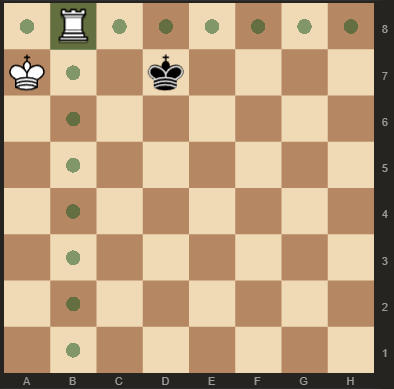
\includegraphics[width=\textwidth]{images/krk_move.png}    \end{figure}
  \end{column}
\end{columns}

\end{frame}

\begin{frame}[fragile]{MDP: Transition}

  Transition probability $\Pr(S_{t+1}=s' | S_t=s, A_t=a)$ 
  
  \begin{itemize}
    \item \textbf{Oracle Defender}: deterministic evolution

  {\scriptsize\begin{verbatim}
  state.do_move(Move)             // white deterministic
  state.do_move(oracle.reply())   // black deterministic
  \end{verbatim}}
    \item \textbf{Random Defender}: stochastic evolution
    
  {\scriptsize\begin{verbatim}
  state.do_move(Move)               // white deterministic
  state.do_move(random_reply())     // black random
  \end{verbatim}}
  \end{itemize}
  
\end{frame}


\begin{frame}{MDP: Reward}

  \textbf{Goal:} find the fastest mate

  \textbf{Reward:}\footnote{\tiny{Except for Value Iteration}}

  \begin{itemize}
    \item checkmate: +1
    \item draw: -1 (always winning for white)
    \item encourage faster mates 
    \begin{itemize}
      \item step penalty: -2/-0.01
      \item discount factor $\gamma = 1$
    \end{itemize}
  \end{itemize}

\end{frame}